% 1977 年宁夏卷第 11 题：三角形 ABC（C 在上方），三边分别标注 a（BC 边）、b（CA 边）、c（AB 边）（按源卷第 2 页布局）
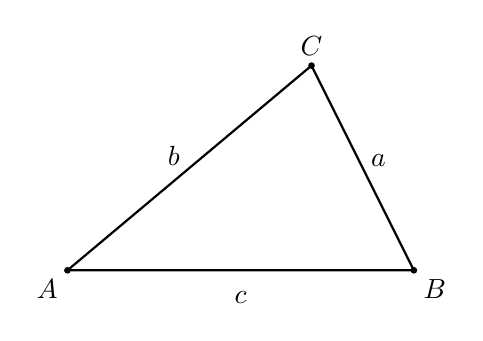
\begin{tikzpicture}[scale=1.0]
  \coordinate (A) at (0,0);
  \coordinate (B) at (4.4,0);
  \coordinate (C) at (3.1,2.6);
  \draw[thick] (A)--(B)--(C)--cycle;
  \fill (A) circle (1.2pt) node[below left] {$A$};
  \fill (B) circle (1.2pt) node[below right] {$B$};
  \fill (C) circle (1.2pt) node[above] {$C$};
  \node at (1.35,1.45) {$b$};
  \node at (3.95,1.4) {$a$};
  \node at (2.2,-0.35) {$c$};
\end{tikzpicture}
